\documentclass[11pt,letter, swedish, english
]{article}
\pdfoutput=1

\usepackage{../custom_as}
\usepackage[makeroom
]{cancel}
\graphicspath{{figures/}}

\swapcommands{\Delta}{\varDelta}
\swapcommands{\Omega}{\varOmega}

%%Drar in tabell och figurtexter
\usepackage[margin=10 pt]{caption}
%%För att lägga in 'att göra'-noteringar i texten
\usepackage{todonotes} %\todo{...}

%%För att själv bestämma marginalerna. 
\usepackage[
%            top    = 2.5cm,
%            bottom = 3cm,
%            left   = 3cm, right  = 3cm
]{geometry}

%%För att ändra hur rubrikerna ska formateras


\renewcommand{\thefootnote}{\fnsymbol{footnote}}

\newcommand{\Tc}{\ensuremath{T_{\text{c}}}}
\newcommand{\eF}{\ensuremath{\epsilon_{\text{F}}}}
\newcommand{\wD}{\ensuremath{\omega_{\text{D}}}}

%\usepackage{tikz}

\begin{document}

%\tikzstyle{every picture}+=[remember picture]
%\tikzstyle{na} = [shape=rectangle,inner sep=0pt,text depth=0pt]



%%%%%%%%%%%%%%%%% vvv Inbyggd titelsida vvv %%%%%%%%%%%%%%%%%

\title{Statistical Physics 2 -- PHYS\,705 \\
Assignment 1}
\author{Andréas Sundström}
\date{\today}

\maketitle

%%%%%%%%%%%%%%%%% ^^^ Inbyggd titelsida ^^^ %%%%%%%%%%%%%%%%%

\section{Mean field magnetic susceptibility}
\renewcommand{\thesubsection}{\arabic{section} (\roman{subsection})}

In this problem, we will study the magnetic susceptibility, $\chi$, in
view of the MFT approach to the Ising model. We will look at the
asymptotic behaviour of $\chi$ for $T\to0^+$ and $T\to\Tc$.

We begin from the MF equation
\begin{equation}\label{eq:1_MFE}
M=\tanh(\frac{MJ + B}{T}),
\end{equation}
and the definition of susceptibility
\begin{equation}\label{eq:1_chi}
\chi:=\eval{\dv{M}{B}}_{B=0}.
\end{equation}

By applying \eqref{eq:1_chi} to \eqref{eq:1_MFE}, we get
\begin{equation}
\chi=\frac{1}{\cosh^2(MJ/T)}\, 
\qty(\frac{J}{T}\chi+\frac{1}{T}),
\end{equation}
or in other words
\begin{equation}\label{eq:1_chi_exact}
\chi=\frac{1}{T\cosh^2(MJ/T)-\Tc}.
\end{equation}
In the last step we also used the fact that $\Tc=J$ using the MFT approach.

\subsection{Zero temperature limit}
As $T\to0^+$, the leading order behaviour of the hyperbolic cosine is
\begin{equation}
\cosh^2\qty(\frac{MJ}{T})\sim \frac{1}{4}\exp(2\frac{\abs{M}J}{T}).
\end{equation}
This exponential growth will dominate over the factor $T$ in
front and the constant $-\Tc$ in the denominator. And \eqref{eq:1_MFE}
also shows us that $M\to\pm1$ as $T\to0^+$. 

The asymptotic behaviour of \eqref{eq:1_chi_exact} will be 
\begin{equation}
\chi\sim \frac{4}{T}\exp(-2\frac{J}{T})
\qcomma \text{as}\ T\to0.
\end{equation}
And to be clear, this asymptotic behaviour results in $\chi(T)\to0$ as
$T\to0$. 


\subsection{Critical temperature limit}






\section{Phase transitions in Landau theory}
\renewcommand{\thesubsection}{\arabic{section} (\alph{subsection})}
\renewcommand{\thesubsubsection}{\arabic{section} (\alph{subsection},\,\roman{subsubsection})}

Here, we will use the Landau free energy
\begin{equation}
F=-bM+tM^2+uM^4+M^6,
\end{equation}
where $b=B/T$, $t=(T-\Tc)/\Tc$ and $u$ is some coefiicient with no
restrictions. 

\subsection{Generic forms of $F$}
There will be, depending on how precise you want to be, around four
different generic forms of $F$, and they occur at
\begin{enumerate}[label=\Roman*.]
\item $t\ge0$, $u\ge0$ %$\quad\Longrightarrow\quad$ just one minimum at $M=0$
\item $t<0$, $u$ any value; or $t=0$, $u<0$
%$\quad\Longrightarrow\quad$ local maximum at $M=0$ and two minimums with $M^2{>}\,0$.
\item $0<t<u^2/4$, $u<0$
\item $t>u^2/4$, $u<0$
\end{enumerate}
These four cases encompass all of the $u{-}T$ plane. The generic forms
of $F(M)$ can be seen in 

\begin{figure}
\centering
% GNUPLOT: LaTeX picture with Postscript
\begingroup
  \makeatletter
  \providecommand\color[2][]{%
    \GenericError{(gnuplot) \space\space\space\@spaces}{%
      Package color not loaded in conjunction with
      terminal option `colourtext'%
    }{See the gnuplot documentation for explanation.%
    }{Either use 'blacktext' in gnuplot or load the package
      color.sty in LaTeX.}%
    \renewcommand\color[2][]{}%
  }%
  \providecommand\includegraphics[2][]{%
    \GenericError{(gnuplot) \space\space\space\@spaces}{%
      Package graphicx or graphics not loaded%
    }{See the gnuplot documentation for explanation.%
    }{The gnuplot epslatex terminal needs graphicx.sty or graphics.sty.}%
    \renewcommand\includegraphics[2][]{}%
  }%
  \providecommand\rotatebox[2]{#2}%
  \@ifundefined{ifGPcolor}{%
    \newif\ifGPcolor
    \GPcolortrue
  }{}%
  \@ifundefined{ifGPblacktext}{%
    \newif\ifGPblacktext
    \GPblacktexttrue
  }{}%
  % define a \g@addto@macro without @ in the name:
  \let\gplgaddtomacro\g@addto@macro
  % define empty templates for all commands taking text:
  \gdef\gplbacktext{}%
  \gdef\gplfronttext{}%
  \makeatother
  \ifGPblacktext
    % no textcolor at all
    \def\colorrgb#1{}%
    \def\colorgray#1{}%
  \else
    % gray or color?
    \ifGPcolor
      \def\colorrgb#1{\color[rgb]{#1}}%
      \def\colorgray#1{\color[gray]{#1}}%
      \expandafter\def\csname LTw\endcsname{\color{white}}%
      \expandafter\def\csname LTb\endcsname{\color{black}}%
      \expandafter\def\csname LTa\endcsname{\color{black}}%
      \expandafter\def\csname LT0\endcsname{\color[rgb]{1,0,0}}%
      \expandafter\def\csname LT1\endcsname{\color[rgb]{0,1,0}}%
      \expandafter\def\csname LT2\endcsname{\color[rgb]{0,0,1}}%
      \expandafter\def\csname LT3\endcsname{\color[rgb]{1,0,1}}%
      \expandafter\def\csname LT4\endcsname{\color[rgb]{0,1,1}}%
      \expandafter\def\csname LT5\endcsname{\color[rgb]{1,1,0}}%
      \expandafter\def\csname LT6\endcsname{\color[rgb]{0,0,0}}%
      \expandafter\def\csname LT7\endcsname{\color[rgb]{1,0.3,0}}%
      \expandafter\def\csname LT8\endcsname{\color[rgb]{0.5,0.5,0.5}}%
    \else
      % gray
      \def\colorrgb#1{\color{black}}%
      \def\colorgray#1{\color[gray]{#1}}%
      \expandafter\def\csname LTw\endcsname{\color{white}}%
      \expandafter\def\csname LTb\endcsname{\color{black}}%
      \expandafter\def\csname LTa\endcsname{\color{black}}%
      \expandafter\def\csname LT0\endcsname{\color{black}}%
      \expandafter\def\csname LT1\endcsname{\color{black}}%
      \expandafter\def\csname LT2\endcsname{\color{black}}%
      \expandafter\def\csname LT3\endcsname{\color{black}}%
      \expandafter\def\csname LT4\endcsname{\color{black}}%
      \expandafter\def\csname LT5\endcsname{\color{black}}%
      \expandafter\def\csname LT6\endcsname{\color{black}}%
      \expandafter\def\csname LT7\endcsname{\color{black}}%
      \expandafter\def\csname LT8\endcsname{\color{black}}%
    \fi
  \fi
  \setlength{\unitlength}{0.0500bp}%
  \begin{picture}(9070.00,8502.00)%
    \gplgaddtomacro\gplbacktext{%
      \csname LTb\endcsname%
      \put(192,6220){\rotatebox{-270}{\makebox(0,0){\strut{}$F(M, t, u)$}}}%
      \put(2267,4419){\makebox(0,0){\strut{}$M$}}%
      \put(2267,8141){\makebox(0,0){\strut{}I. $t\ge0$, $u\ge0$}}%
    }%
    \gplgaddtomacro\gplfronttext{%
    }%
    \gplgaddtomacro\gplbacktext{%
      \csname LTb\endcsname%
      \put(4727,6220){\rotatebox{-270}{\makebox(0,0){\strut{}$F(M, t, u)$}}}%
      \put(6802,4419){\makebox(0,0){\strut{}$M$}}%
      \put(6802,8141){\makebox(0,0){\strut{}II. $t<0$, $u$ any value; or $t=0$, $u<0$}}%
    }%
    \gplgaddtomacro\gplfronttext{%
    }%
    \gplgaddtomacro\gplbacktext{%
      \csname LTb\endcsname%
      \put(192,1969){\rotatebox{-270}{\makebox(0,0){\strut{}$F(M, t, u)$}}}%
      \put(2267,168){\makebox(0,0){\strut{}$M$}}%
      \put(2267,3891){\makebox(0,0){\strut{}III. $0<t<u^2/4$, $u<0$}}%
    }%
    \gplgaddtomacro\gplfronttext{%
    }%
    \gplgaddtomacro\gplbacktext{%
      \csname LTb\endcsname%
      \put(4727,1969){\rotatebox{-270}{\makebox(0,0){\strut{}$F(M, t, u)$}}}%
      \put(6802,168){\makebox(0,0){\strut{}$M$}}%
      \put(6802,3891){\makebox(0,0){\strut{}IV. $t>u^2/4$, $u<0$}}%
    }%
    \gplgaddtomacro\gplfronttext{%
      \csname LTb\endcsname%
      \put(7854,891){\makebox(0,0)[r]{\strut{}$t>u^2/4$, but not by much}}%
      \csname LTb\endcsname%
      \put(7854,651){\makebox(0,0)[r]{\strut{}$t\gg u^2/4$}}%
    }%
    \gplbacktext
    \put(0,0){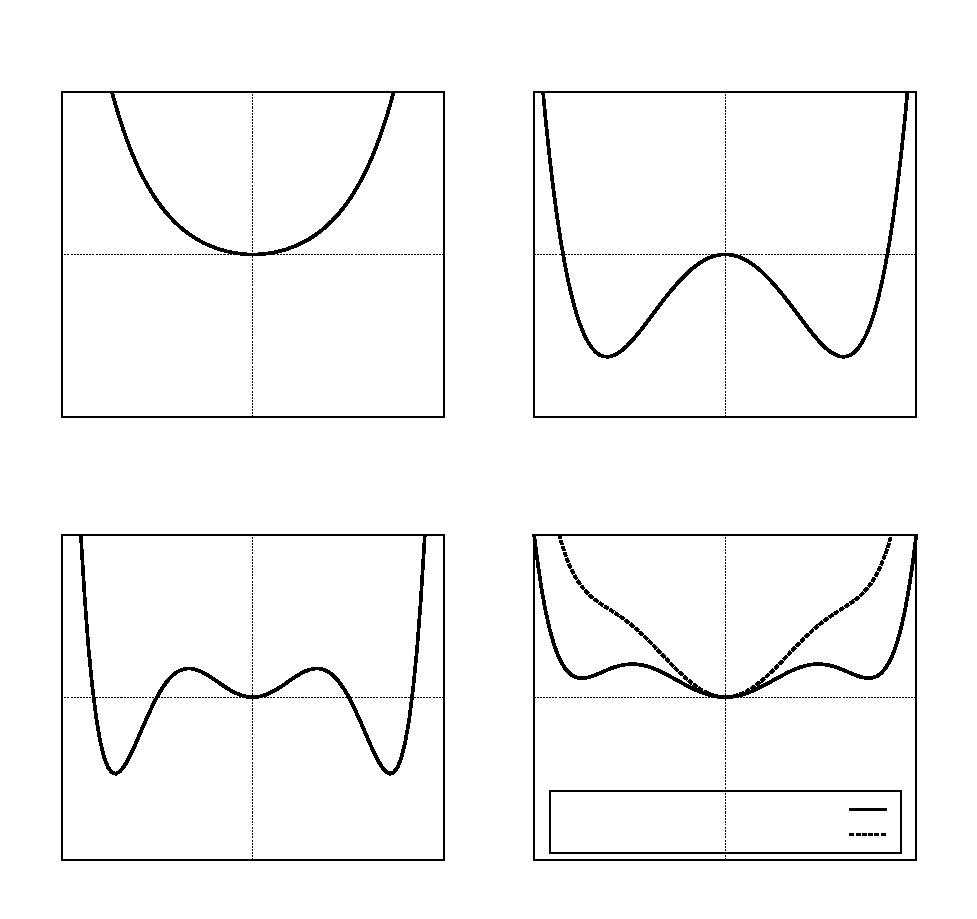
\includegraphics{generic_forms}}%
    \gplfronttext
  \end{picture}%
\endgroup

\caption{}
\label{fig:2a}
\end{figure}







\section{1D Ising model}



\section{Ising model generalization}





\end{document}




%  LocalWords:  MFT MF
